\section{Design}
\label{sec:design}

In order to permit applications to \textit{fully leverage the 10s of $\mu{}s$
latencies available from the latest datacenter networks}, we propose a novel design
for serverless platforms that runs user-submitted microservices within shared
processes.  This structure is possible thanks to our combined use of
\textit{compile-time memory safety guarantees} and \textit{extremely fine-grained
preemption}.  To the best of our knowledge, we are the first system to combine these
two building blocks to create a system that is able to deliver single-digit
invocation latency for lightweight, short-lived tasks.

Our system comprises (1) a central dispatch process that manages the compute node,
receiving requests and assigning them to (2) a number of worker processes (one per
dedicated compute core) via a shared memory region.  Each worker process runs a
tight loop that polls on a ready bit in shared memory; once it finds work to be done,
it sets itself up to catch any runtime panic and jumps into user code.  The worker
process receives frequent \texttt{SIGALRM}s to ensure it never loses control of its
CPU:\ in the associated handler, it checks how for long the current job has been
running and ends any that has gone over budget.  The rest of this section covers the
trust model and the preemption scheme.

\paragraph{Trust model}
Users submit their microservices in the form of Rust source code, allowing the
serverless operator to pass the \texttt{-Funsafe-code} flag while compiling to reject
any \texttt{unsafe} code.  This process doesn't need to be performed on the compute
nodes so long as the deployment server tasked with compilation runs the same version
of the Rust compiler\footnote{This restriction exists because, as of the latest
release (1.23.0) of the compiler, Rust doesn't have a stable ABI.}.  The operator
needs to trust the compiler, standard library, and any libraries against which it
will permit the microservice to link, but importantly need not worry about the
microservice itself.  We believe that most users would find it acceptable to be
presented with a list of permissible dependencies.  Any libraries that make no use of
\texttt{unsafe} code can be whitelisted without review, and to approximate how big
such a list would be given the current Rust ecosystem, we turn to a 2017
study~\cite{www-cratesio-unsafe} by the Tock authors that found just under half of
the Rust package manager's top 1000 most-downloaded libraries to be free of
\texttt{unsafe} code.  They caution that many of those packages have unsafe
dependencies, but we suspect that reviewing a relatively small number of popular
libraries would open up the majority of the most popular packages.

After a microservice is compiled to a shared object file, it should be distributed to
each compute node on which it might run.  Then, in order to ensure that invokers will
experience the warm-start latencies discussed in Section~\ref{sec:motive}, those
nodes' dispatchers should instruct one or more of their workers to preload the
dynamic library.  In the event that the provider experiences too many active
microservices for its available resources, it can unload some libraries; on their
next invocation, they will experience invocation latency greater than the network
latency, but comparable to the \textit{warm-start} latencies of today's serverless
systems.

\paragraph{Preemption scheme}
The system must be able to detect and recover from microservices that, whether
maliciously or negligently, attempt to run for longer than permitted.  The two parts
of this problem are (1) regaining control of the CPU and (2) aborting and cleaning up
after the user code.

As proposed in Section~\ref{sec:motive}, regaining control of the CPU happens when a
\texttt{SIGALRM} from the kernel transfers control to the worker process's signal
handler.  The handler then checks how long the current microservice has been running
and decides whether it should be killed.  The remaining questions are:  ``For how
long should each microservice be allowed to run?'' and ``How often should the handler
execute (the \textbf{quantum})?''

Let us consider the impact of microservice runtime on tail latency in a well-utilized
but not overloaded compute node, which we'll consider to be one where there is a user
task executing on each available core, but no backlog behind which an incoming task
must wait.  (This being preliminary work, any discussion of the cluster-level
scheduling responsible for these theoretical conditions are outside the scope of
this paper.)  Furthermore, we'll assume an incoming microservice that is warm on each
worker thread.  We define $L$ to be the desired invocation latency, $B$ to be the
compute budget allotted to each microservice, and $r_c$ to be the remaining runtime
of the microservice on CPU $c$.  Thus, in the worst case (where all tasks are
executing for their entire allotted time) the probability that the incoming
microservice will have somewhere to run in time to meet the latency SLO is given by:
\begin{equation}
p(r_\textrm{min} \le L) = \sum\limits_{c \in C} p(r_c \le L) = \big| C \big| \frac{L}{B}
\end{equation}
Given the 14 cores in our setup and imagining we want to keep the 99\% tail
($p(r_\textrm{min} \le L) = 0.99$) to an $L$ of 8 $\mu{}s$, we need to kill tasks
running for more than 113 $\mu{}s$.

We showed at the end of Section~\ref{sec:motive} that this is easily
\textit{achievable}, but can it be done \textit{efficiently}?  To find out, we wrote
a microservice that measures the throughput of computing SHA-512 hashes over 64 B of
data at a time.  We then subjected its worker process to \texttt{SIGALRM}s, varying
the quantum and observing the effect on the hashing throughput.
Figure~\ref{fig:hashtput} demonstrates that by a quantum of about 20 $\mu{}s$,
throughput had reached 90\% of baseline.  Considering this an acceptable performance
degradation, we adopt this quantum and prescribe a runtime budget of 93 $\mu{}s$ so
that we can always kill over-budget microservices in time to avoid impacting the tail
latency.

\begin{figure}
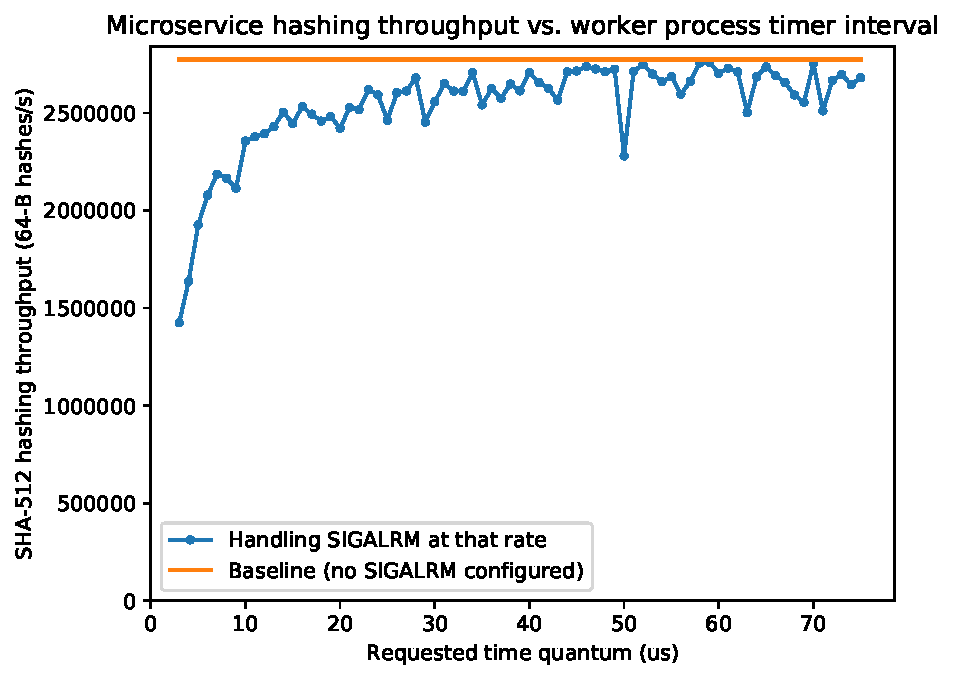
\includegraphics[width=\columnwidth]{figs/2018-02-02-evaluation_quantum-hasher_throughput-throughput}
\caption{Effect of \texttt{SIGALRM} quantum on SHA hashing throughput}
\label{fig:hashtput}
\end{figure}

The problem of regaining control addressed, we now discuss the mechanism for aborting
and cleanup.  POSIX signal handlers receive as one of their arguments a pointer to a
\texttt{ucontext\_t} structure containing a snapshot of the process's PCB (process
control block) the moment before it received the signal.  The most na\"ive way to
regain control would be to reset the GPRs (general-purpose registers) in this
structure to values recorded just before the worker's tight scheduling loop.  The
problem with this approach is that none of the microservice's state or memory
allocations would be expunged from the worker.

One of the few heavyweight components of the Rust runtime is panic handling, which is
reminiscent of C++'s exception handling.  The compiler inserts landing pads into each
function that call the destructors for its variables, and if the program ever panics,
the standard library unwinds the stack, jumping to each landing pad in turn.  We
co-opt this functionality by using the \texttt{SIGALRM} handler to change the context
to describe executing a function that raises an explicit panic in a fake stack frame
just above the real top of the stack.

Note that there are several limitations and security ramifications of our current
approach that would need to be addressed before it was safe to use in a production
environment; for details, see Section~\ref{sec:future}.
